\chapter{LogicNet4HEP}\label{ch:fpganet4hep}
\openepigraph{The Europeans and the Americans are not throwing \$10 billion down this gigantic tube for nothing. We're exploring the very forefront of physics and cosmology with the Large Hadron Collider because we want to have a window on creation, we want to recreate a tiny piece of Genesis to unlock some of the greatest secrets of the universe.}{Michio Kaku}
% \section{Task}
The LHC (Large Hadron Collider) is the worlds highest energy particle accelerator. Proton bunches collide at a frequency of 40 MHz, with data-rates in excess of hundreds of terabytes per second. The process of tagging and filtering data at real time is called triggering. Triggering helps reduce data to manageable levels for processing offline. At the CMS detector, this triggers is performed at two stages. The first stage typically uses custom hardware like ASICs or FPGAs~\cite{Duarte_2018} to handle the initial data rates with latency in the range of a few hundres of nano seconds. The second level of triggering, known as High Level Triggering (HLT) uses commercial CPUs to process filtered data in software with longer processing times. We borrow some definitions from the work of Javier Duarte\cite{Duarte_2018} to formalize the task in this section.\\

\marginpar{\centering
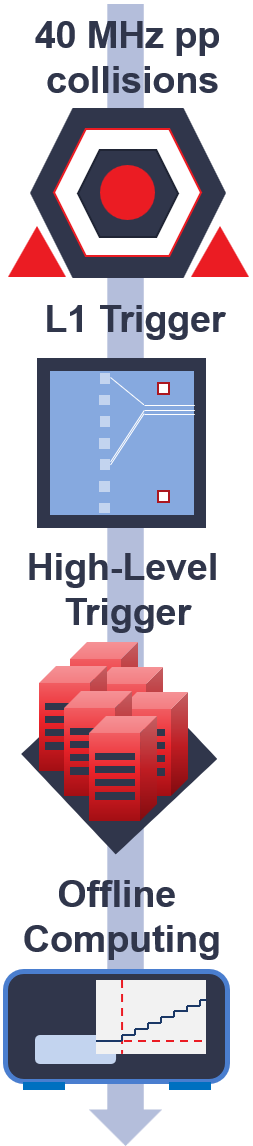
\includegraphics[width=70pt]{figures/bison/LHCdataflow.png}
\captionof{figure}{The LHC big data problem.}
\label{fig:lhcdataflow}
% \endgroup
}

Jets are collimated showers of particles that are created from the decay and hadronziation of quarks $q$ and gluons $g$. Due to the high collision energy at LHC, jet signatures of interest emergy from overlapping quark-initiated showers produced in the decays of heavy standard model particles.
In this task, we focus on the task of classifying a jet as either a quark ($q$), gluon ($g$), W boson ($W$), Z boson ($Z$) or top quark ($t$) jet. 
\newthoughtpar{Key Metrics}
To create an optimal L1 trigger that satisfies the require  ments of the target algorithm, we list the three key metrics considered by~\cite{Duarte_2018}. 
\begin{itemize}
    \item \textbf{Latency}: The total time (usually in units of "clocks") for a single forward pass through the neural network.
    \item \textbf{Initiation Interval}: The number of clock cycles before the neural network can accept a new input. Inference rate is inversely proportional to the initiation interval. This is of key importance as the data should be pipe-lined at the rate of the initiation interval.
    \item \textbf{Resource Usage}: This may encompass the counts of a range of components available on the target FPGA fabric. Some of which may be Block RAMs (BRAMs), Digital Signal Processing Blocks (DSPs), Registers, Lookup-Tables (LUTs).
\end{itemize}
% \section{Models}
\newthoughtpar{Models}
As LogicNet style topologies are quite unique in the heavy sparsity and quantization they desire, we had to do extensive topology exploration to gain insights into how we can get the most performant networks with the lowest resource cost.
\newthoughtpar{Neural Architecture Search}
We considered Neural Architecture Search to find efficient topologies. Neural Architecture Search is a method for automating the design of Neural Networks. There are many ways to define the search space, strategy and getting a performance estimation for evaluating a discovered architecture. In our case, it makes sense to treat neurons as individiual blocks, and discovering not only the hierarchical connectivity, but aiming to discover completely unstructured (not layered) topologies. On top of this, we also have to define a search space carefully. Here, the search space is not only limited to the bit-width and connectivity per neuron but also the overall connectivity across layers. The Performance estimation would fairly straightforward, as we have estimates of the resource usage, as well as can easily give an account of the initiation interval and latency. The initiation interval for an LogicNet style topology is 1, and the latency is essentially equal to the number of intermediate activations that are generated, in a layered fashion.
However, due to the combinatorial nature of this problem, we were too constrained to do a Neural Architecture Search. We aimed to prove that LogicNet style structures can deliver performance benefits. It is very much within the scope of future research to integrate NAS into the LogicNet library, and the library itself is being built with the same in mind. 
\begin{figure}[h]
    \centering
    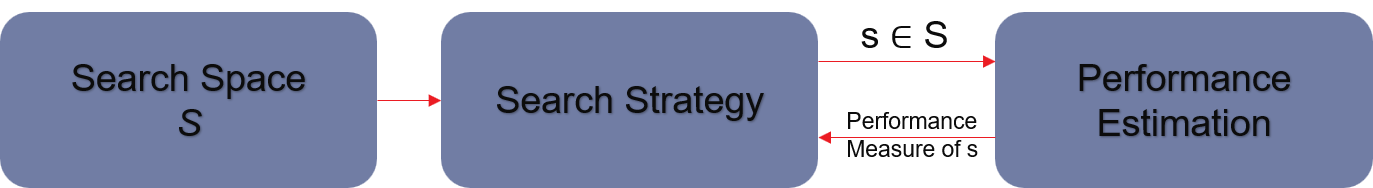
\includegraphics[width=300pt]{figures/bison/NAS.png}
    \caption{Dimensions of the NAS method.}
    \label{fig:NAS}
\end{figure}

\newthoughtpar{Axes of exploration}
As we are exploring LogicNet type topologies by hand, it becomes very important to specify the 'axes of exploration', and make observations along the same lines. For us, there were 3 primary axes of exploration. The Bit-Width of activation, the number of neurons per hidden layer, and the Fan-In (In Bits) per neuron. We have not attempted to explore variable fan-in for neurons with-in a layer. We do however give insights into variable fan-in for individiual layers.


\marginpar{\centering
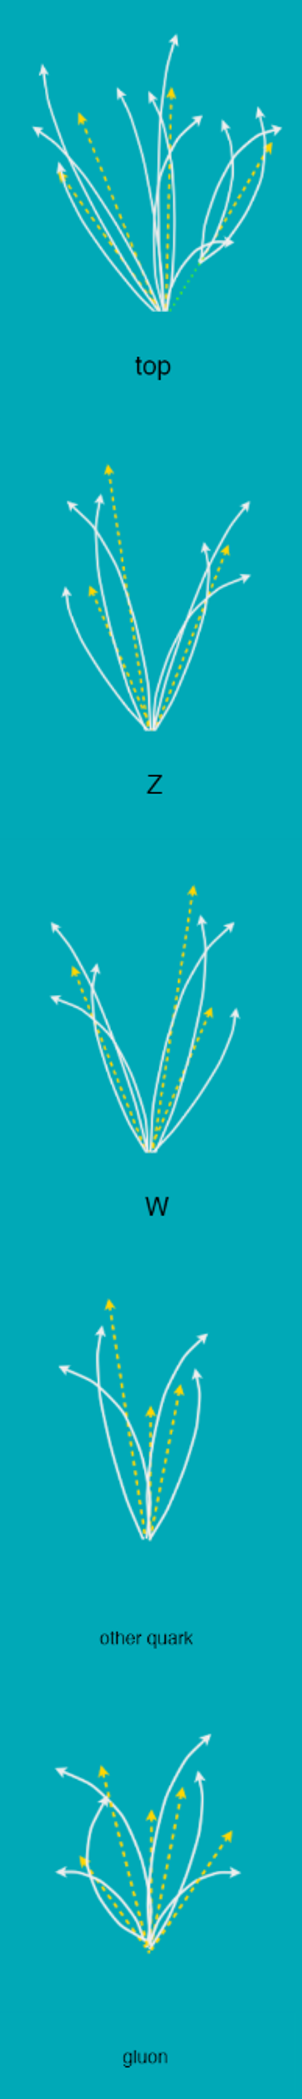
\includegraphics[width=90pt]{figures/bison/classes.png}
\captionof{figure}{Discriminating between highly energetic (boosted) \textbf{\textit{q, g, W, Z, t}} initiated jets. Figure adapted from User: FPGA4HEP on GitHub.}
\label{fig:classesFPGA4HEP}
% \endgroup
}


\newpage

\begin{figure}[h]
    \centering
    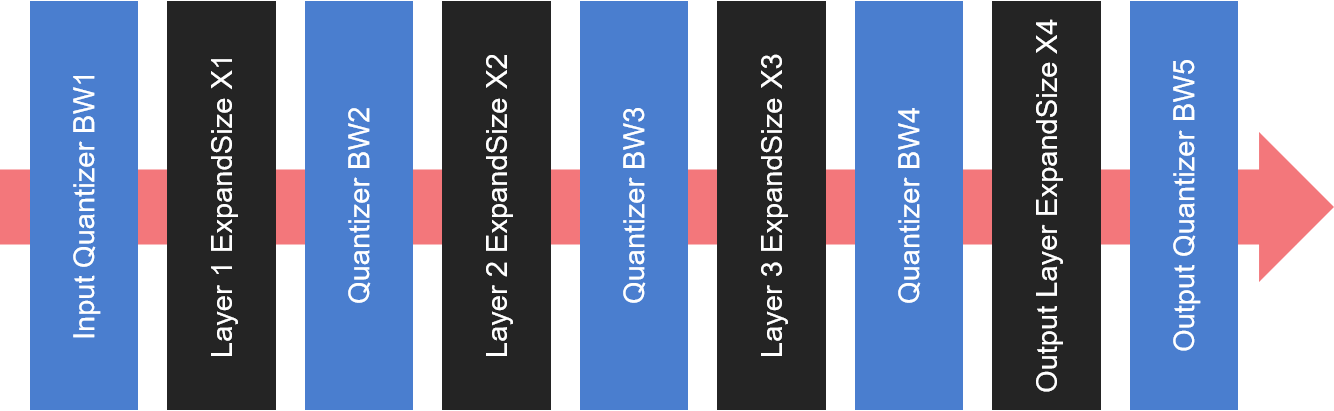
\includegraphics[width=300pt]{figures/bison/FPGA4HEPtopology.png}
    \caption{Our PFGA4HEP Neural Network Architecture.}
    \label{fig:FPGA4HEPtopology}
\end{figure}

\newthoughtpar{Classification performance}
To quantify the performance of the classifier we have made in ~\cref{fig:FPGA4HEPtopology}, we use the same metric sued in~\cite{Duarte_2018}. We use the AUC metric, or area under the Receiver Operating Characteristic (ROC) curve. The ROC curve is given by the background rejection versus signal efficiency computed from sequential cuts on the classifier output, where background rejection is (1 - background efficiency). The Expected AUC is the AUC acheived by a a full 32-bit floating point inference of the neural network. 

\begin{figure}[h]
    \centering
    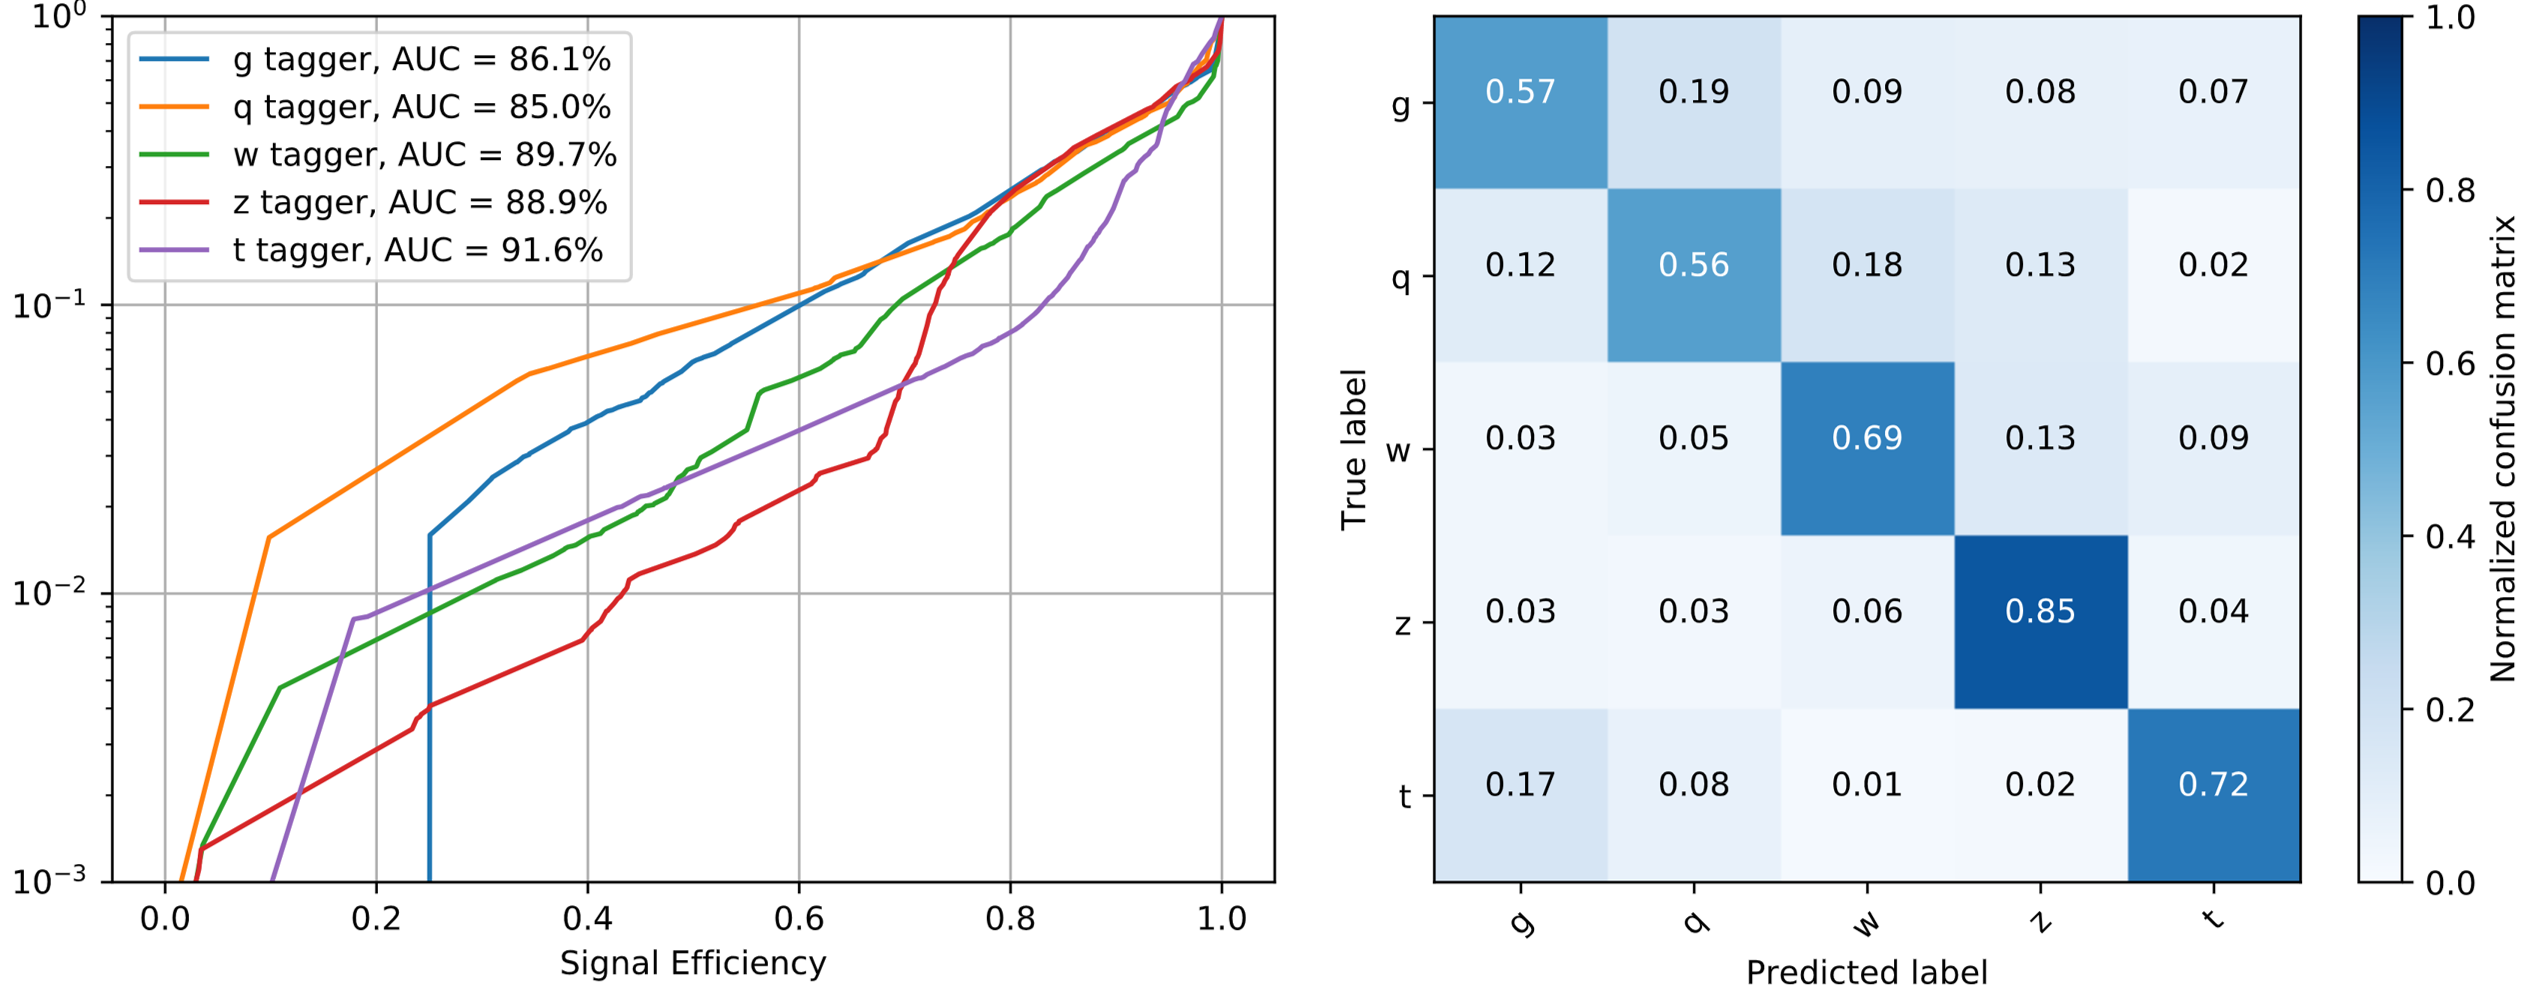
\includegraphics[width=320pt]{figures/bison/classifierperform.png}
    \caption{Performance of the Deep Neural Network Classifier. The Left figure shows the signal efficiency versus the mis-identification rate for q, W, Z, t, g jet identification. The mis-identification rate is based on an equal admixture of the other non-signal jet types. On the right we show the Normalized Confusion Matrix for the classifier.}
    \label{fig:classifierperform}
\end{figure}

\begin{figure}[h]
    \centering
    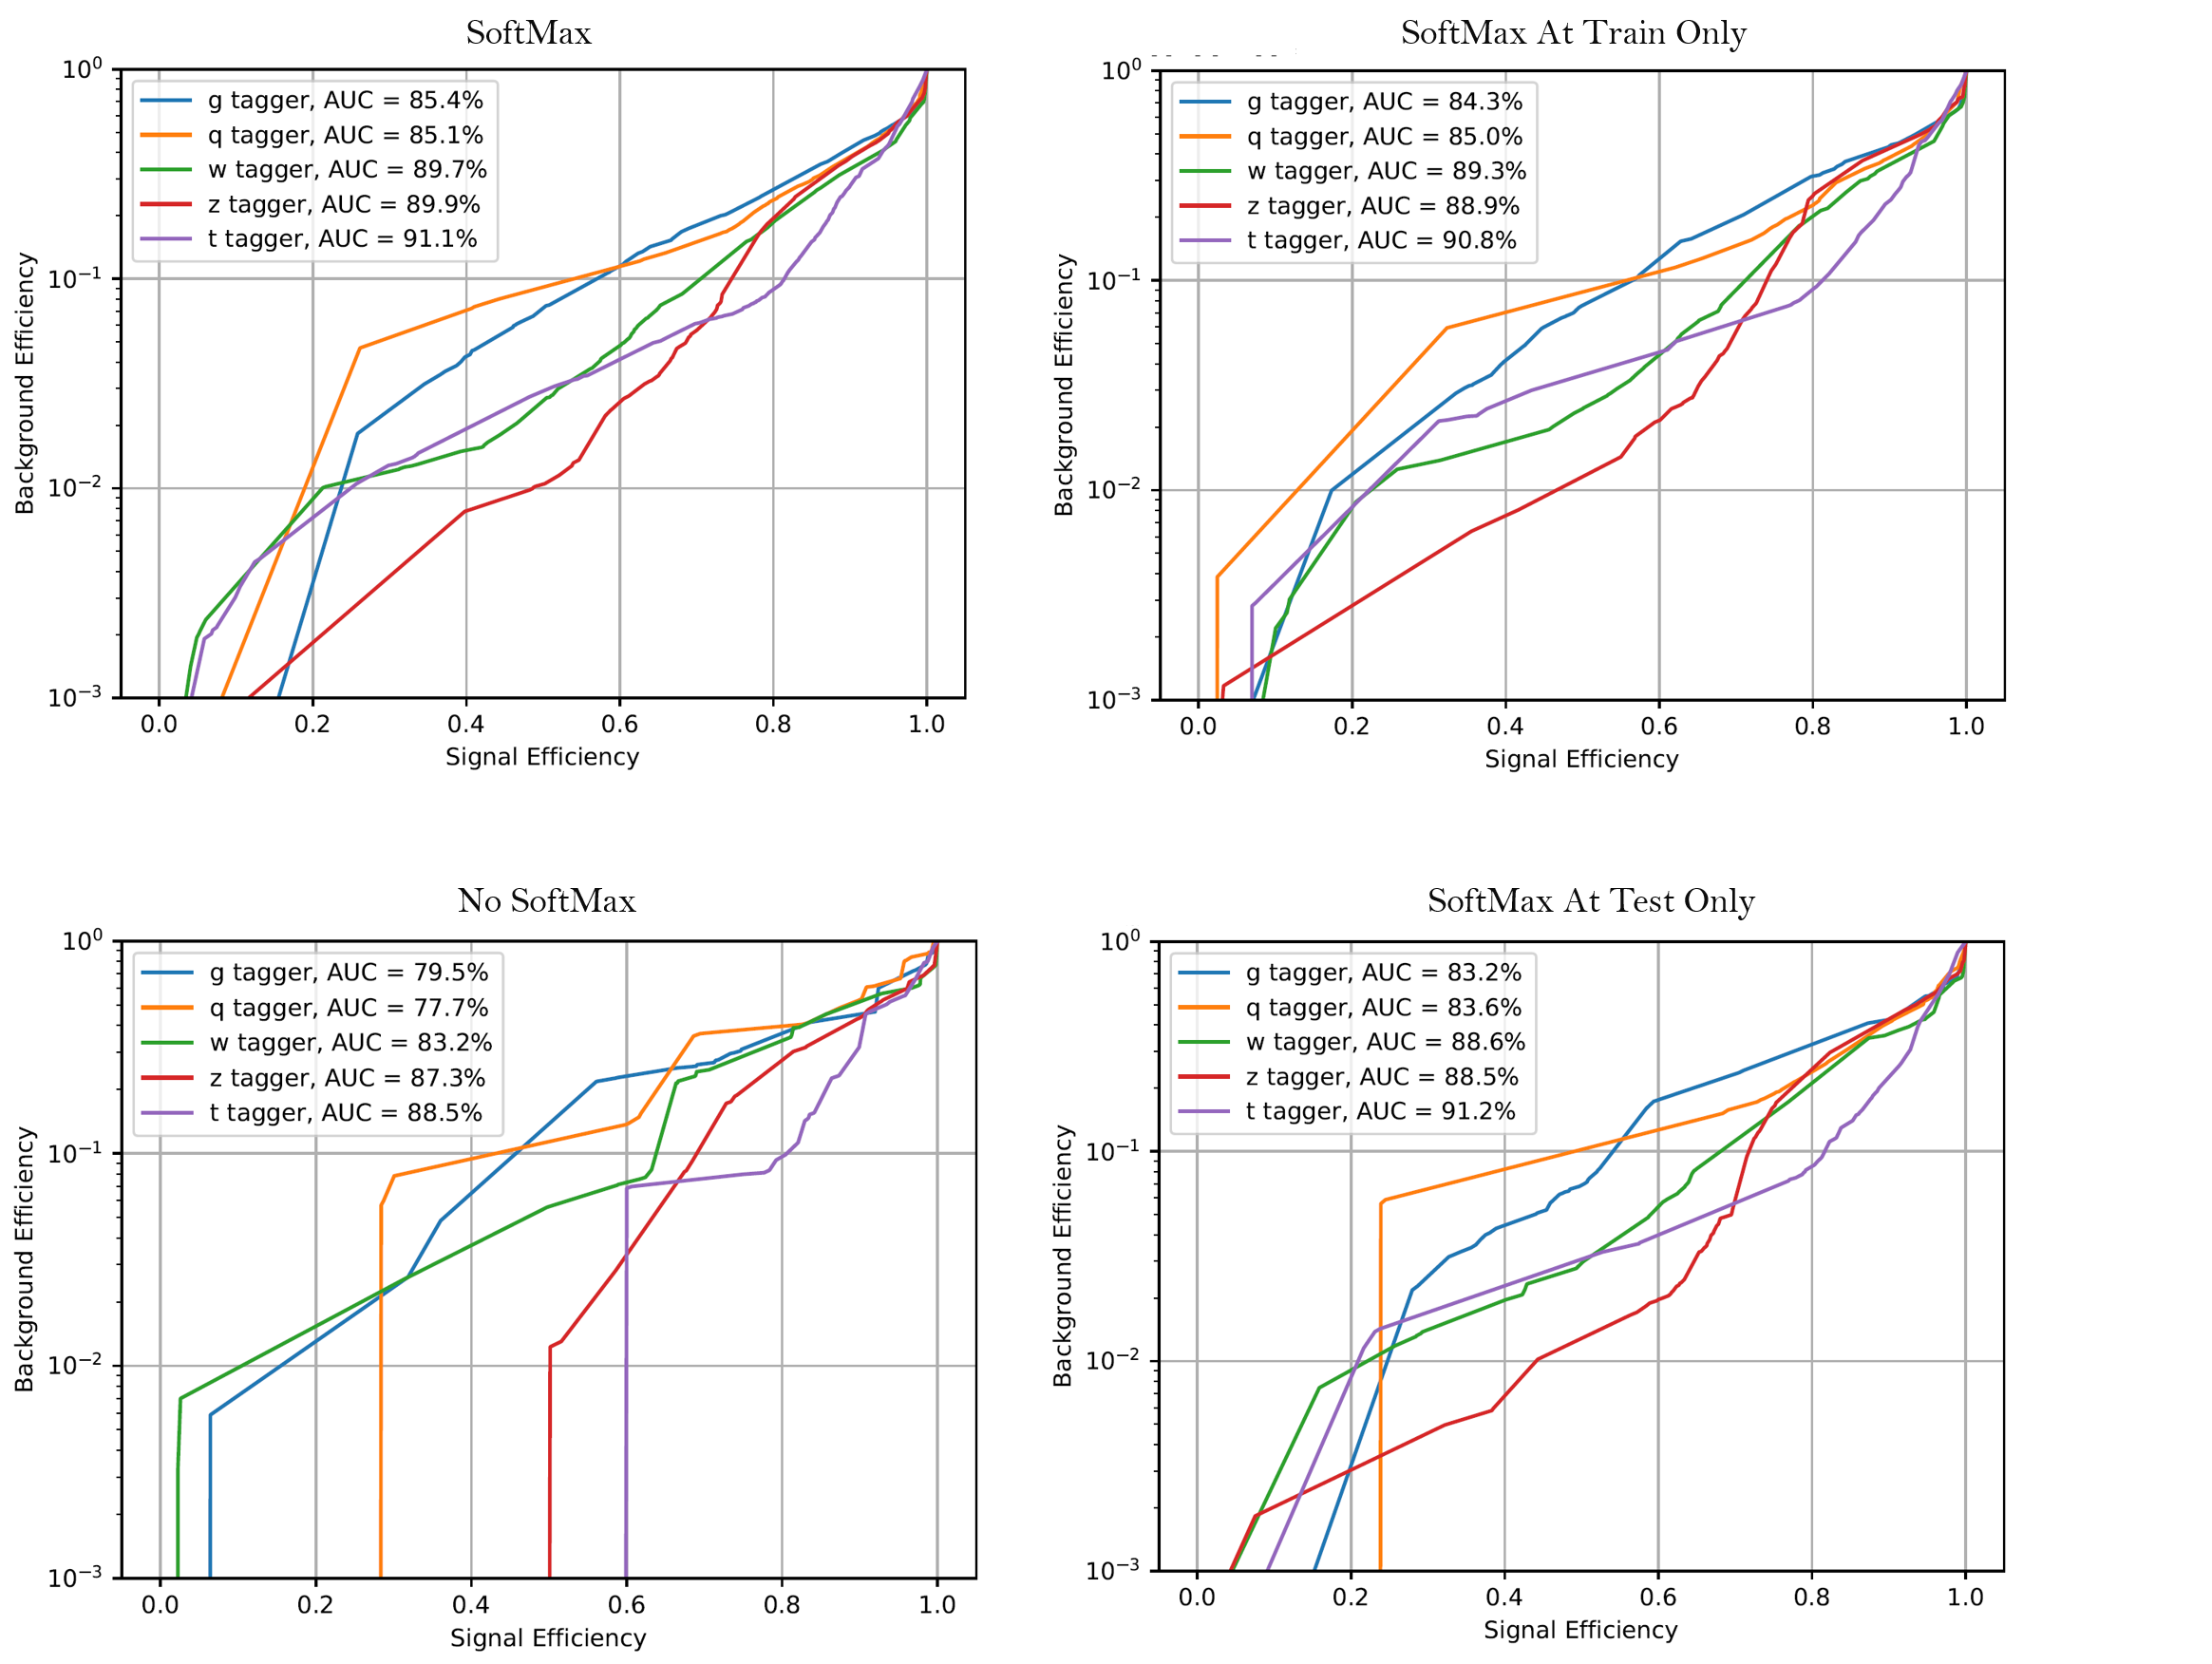
\includegraphics[width=400pt]{figures/bison/SoftMaxTests.png}
    \caption{We train a model on the FPGA4HEP dataset and observe the classifiers Receiver Operating Characteristics with respect to the SoftMax Layer.}
    \label{fig:softmaxtests}
\end{figure}
% \\




\newthoughtpar{Model Descriptions}
It is important to know how we are labelling our models. We refer the users to \cref{fig:FPGA4HEPtopology}. Our models are described in \cref{fpganet4hep:tab:fpga4hepmodels}. The $2^{nd}$ (HL) column can be referred to as $(Neurons_{Layer1}, Neurons_{Layer2}, Neurons_{Layer3})$. The BW refers to the Bit-Width, with X indicating the fan-in of neurons. Note that this fan in is not in bits, but instead the number of 'synapses'. The last layer is special, its bit-width and fan-in are very crucial. Thus, we have specific the fan-in of some models with $X_{fc}$. Where this was not been specified, the final layer would be dense. $BW_{fc}$ refers to the bit-width of the output. This is important as lower bit-width and removal of the SoftMax layer generally results in degradation of the ROC curve. However, the extra cost of a SoftMax layer has been excluded from our analysis.


% \begin{figure}[h]
%     \centering
%     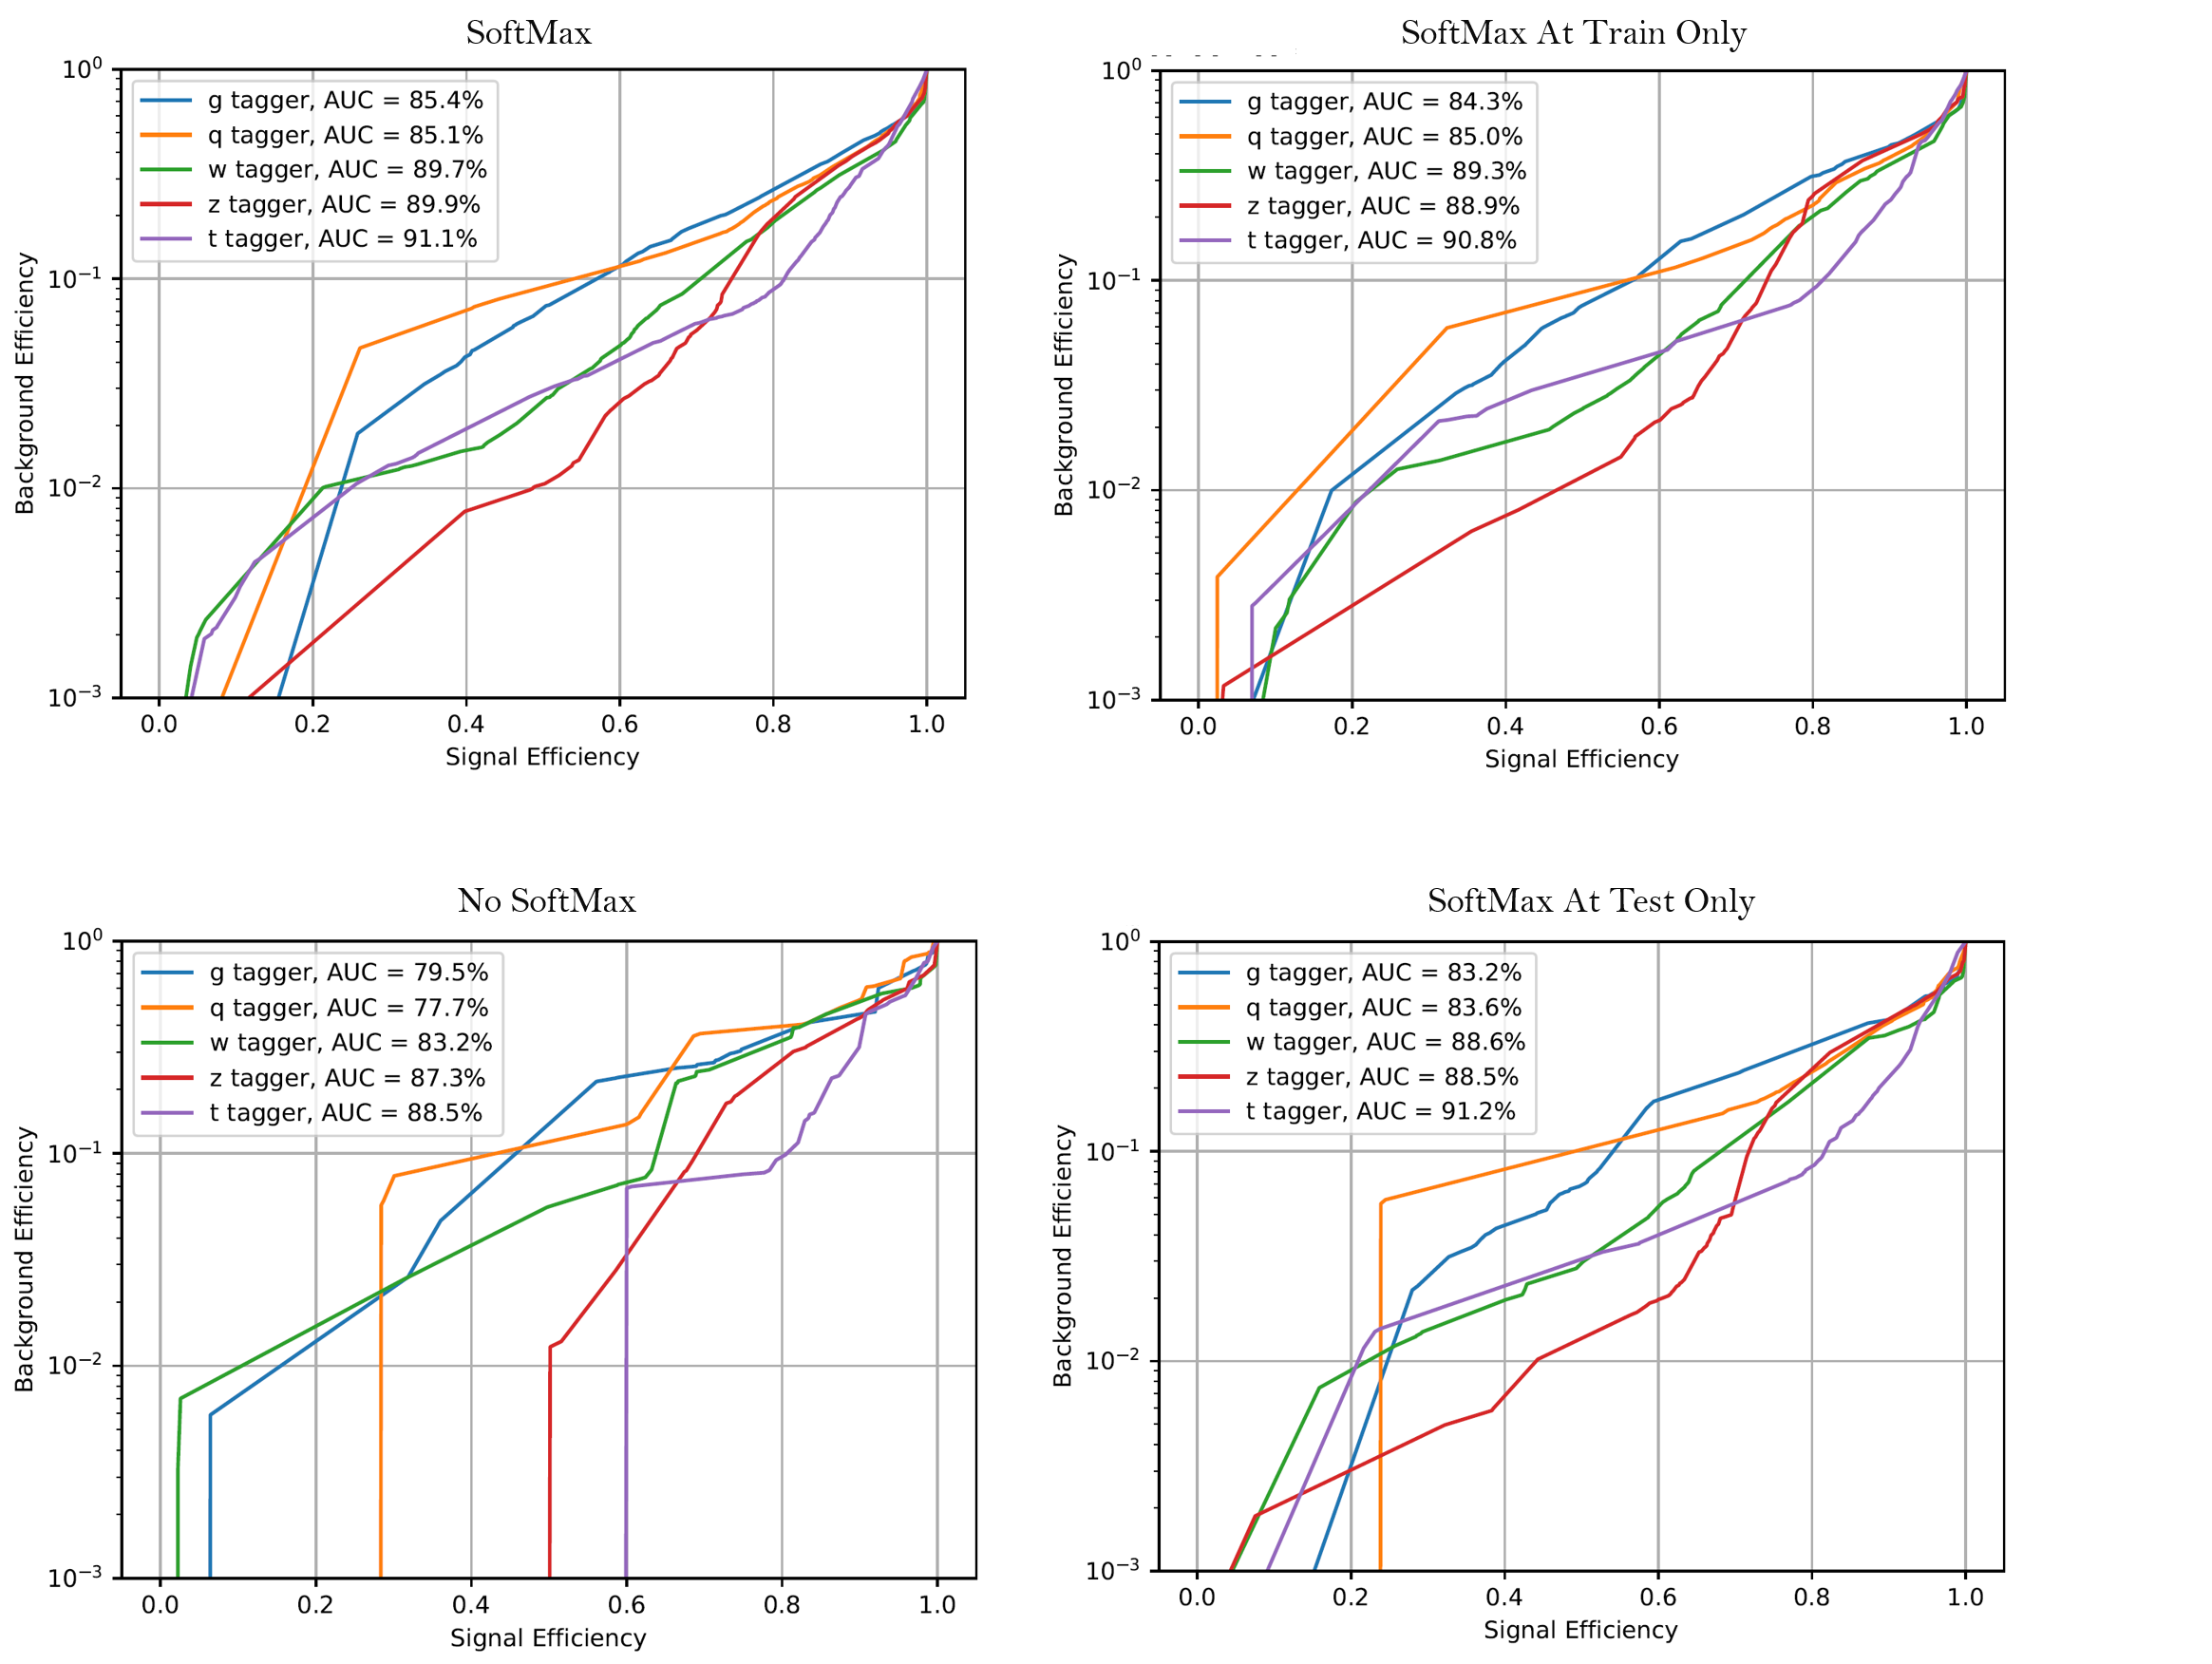
\includegraphics[width=520pt]{figures/bison/SoftMaxTests.png}
%     \caption{We train a model on the FPGA4HEP dataset and observe the classifiers Receiver Operating Characteristics with respect to the SoftMax Layer.}
%     \label{fig:softmaxtests}
% \end{figure}
% % \\


% \newpage
% \input{mainmatter/fpganet4heptable.tex}
% \clearpage

% \input{mainmatter/fpganet4heptable.tex}
% \clearpage
\begin{table}
    \begin{sidecaption}[FPGA4HEP Model List]{%
        Model descriptions
    }[fpganet4hep:tab:fpga4hepmodels]
\begin{threeparttable}
\begin{tabular}{lrrrrrrrrr}
\hline
Model & HL            & BW & X & $X_{fc}$ & $BW_{fc}$   & LUTL1 & LUTL2 & LUTL3 & LUTL4 \\ \hline
A     & (64, 64, 64)  & 3  & 3 & -         & 3          & 2112  & 2112  & 2112  & 4125  \\
B     & (128, 64, 32) & 3  & 3 & -         & 3          & 4224  & 2112  & 1056  & 2090  \\
C     & (64, 32, 32)  & 2  & 3 & -         & 2          & 128   & 64    & 64    & 1415  \\ 
D     & (64, 32, 32)  & 2  & 5 & 6         & 4          & 2688  & 1344  & 1344  & 3400  \\ 
E     & (64, 64, 64)  & 2  & 4 & 4         & 4          & 640   & 640   & 640   & 200   \\\hline 
\end{tabular}
\end{threeparttable}
\end{sidecaption}
\end{table}

\begin{table}
    \begin{sidecaption}[FPGA4HEP Main Table]{%
        Accuracy and LUT costs of some explored models. Note that the LUTs is the estimate described by \eqref{lutcostcloseform}. An in-depth discussion of the closed form equation of cost versus the synthesized cost has been discussed before. Note that the \textbf{g, q, W, Z, t} are reported as Area Under Curve - Receiver Operating Characteristic.
    }[fpganet4hep:tab:fpga4hepresults]
\begin{threeparttable}
\begin{tabular}{lrrrrrrrrrrrrrrrr}
\hline
Model &    g &   q  &   W  &   Z  &   t  & Avg AUC-ROC  & LUTs     & \% FC \\ \hline
A     & 89.3 & 86.2 & 89.8 & 89.3 & 92.7 & 89.46  & 10461    & 39.43 \\
B     & 86.5 & 86.0 & 90.5 & 90.5 & 91.9 & 89.08  & 9482     & 22.04 \\
C     & 85.4 & 82.9 & 84.9 & 83.1 & 90.3 & 85.32  & 1671     & 84.68 \\ 
D     & 85.8 & 85.0 & 89.5 & 89.2 & 91.5 & 88.20  & 8776     & 38.74 \\ 
E     & 86.5 & 85.4 & 90.0 & 89.6 & 92.0 & 88.70  & 2120     & 9.43  \\\hline 
    \end{tabular}
\end{threeparttable}
\end{sidecaption}
\end{table}

% \marginpar{\centering
% 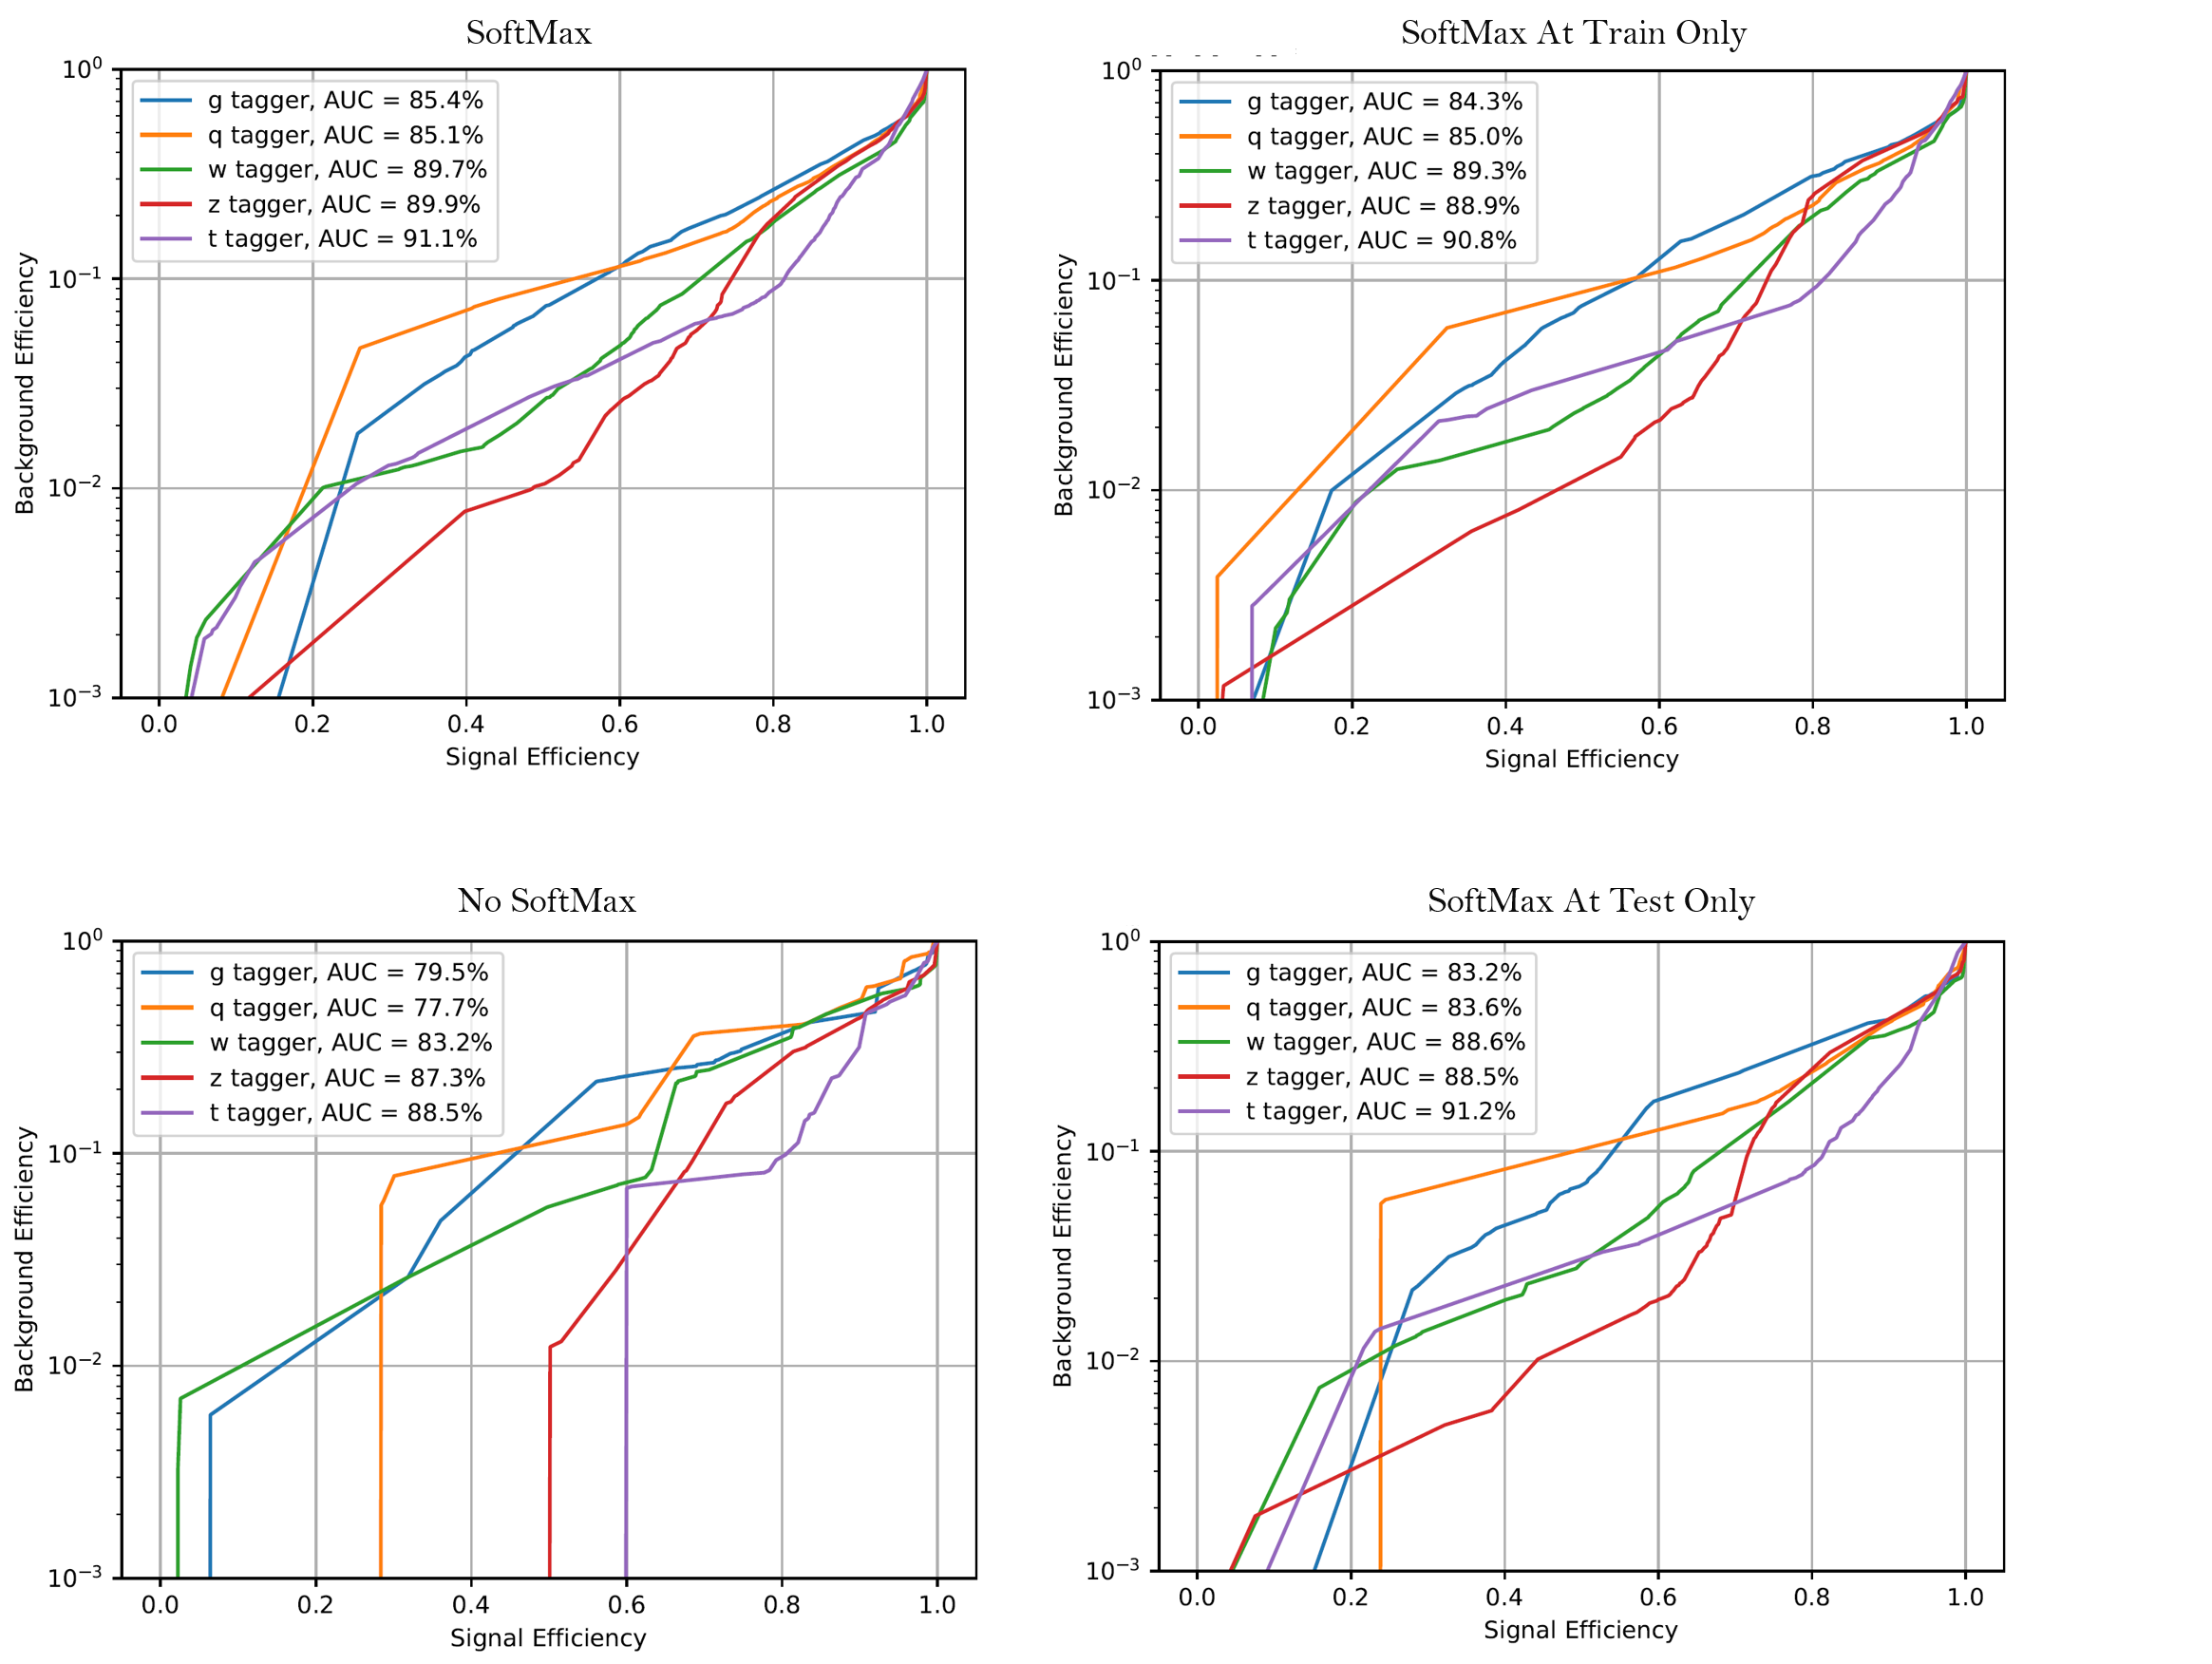
\includegraphics[width=520pt]{figures/bison/SoftMaxTests.png}
% \captionof{figure}{We train a model on the FPGA4HEP dataset and observe the classifiers Receiver Operating Characteristics with respect to the SoftMax Layer.}
% \label{fig:softmaxtests}
% % \endgroup
% }
% % \vspace{520pt}

\begin{figure}[h]
    \centering
    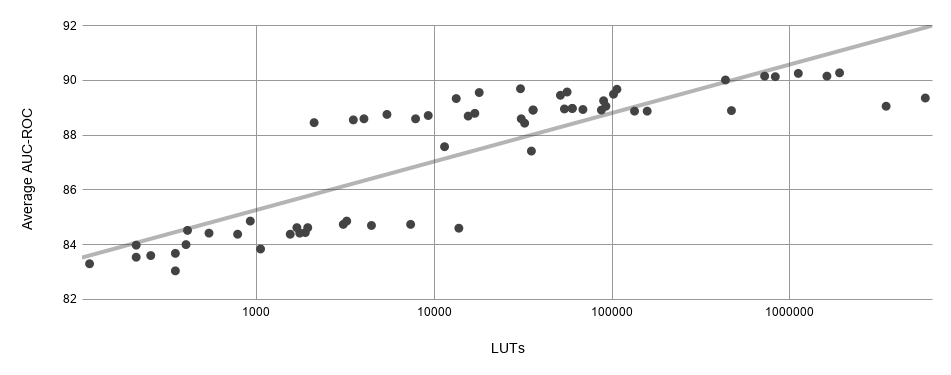
\includegraphics[width=350pt]{figures/bison/LUTvAcc.png}
    \caption{Increase in Accuracy with increase in LUT cost.}
    \label{fig:lutvacc}
\end{figure}

\begin{figure}[h]
    \centering
    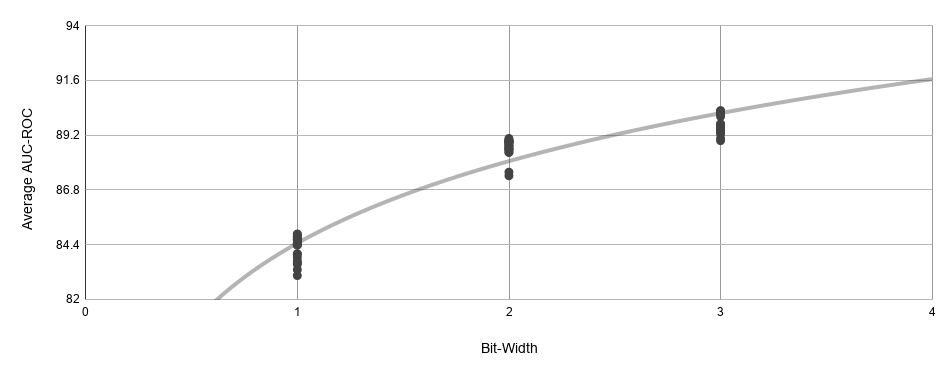
\includegraphics[width=350pt]{figures/bison/BWvAcc.png}
    \caption{Increase in Accuracy with increase in Bit-Width.}
    \label{fig:BWvacc}
\end{figure}

\newthoughtpar{Performance with and without SoftMax}
In the previous section, we described our models and briefly touched upon the effect of SoftMax on ROC. Not only does the SoftMax make the training better, it makes the classifier more robust to noise. While the effects of removing the SoftMax layer after training is not evident on the confusion matrix, upon graphing the ROC, it becomes important to inspect it more closely.
% \begin{figure}[h]
%     \centering
%     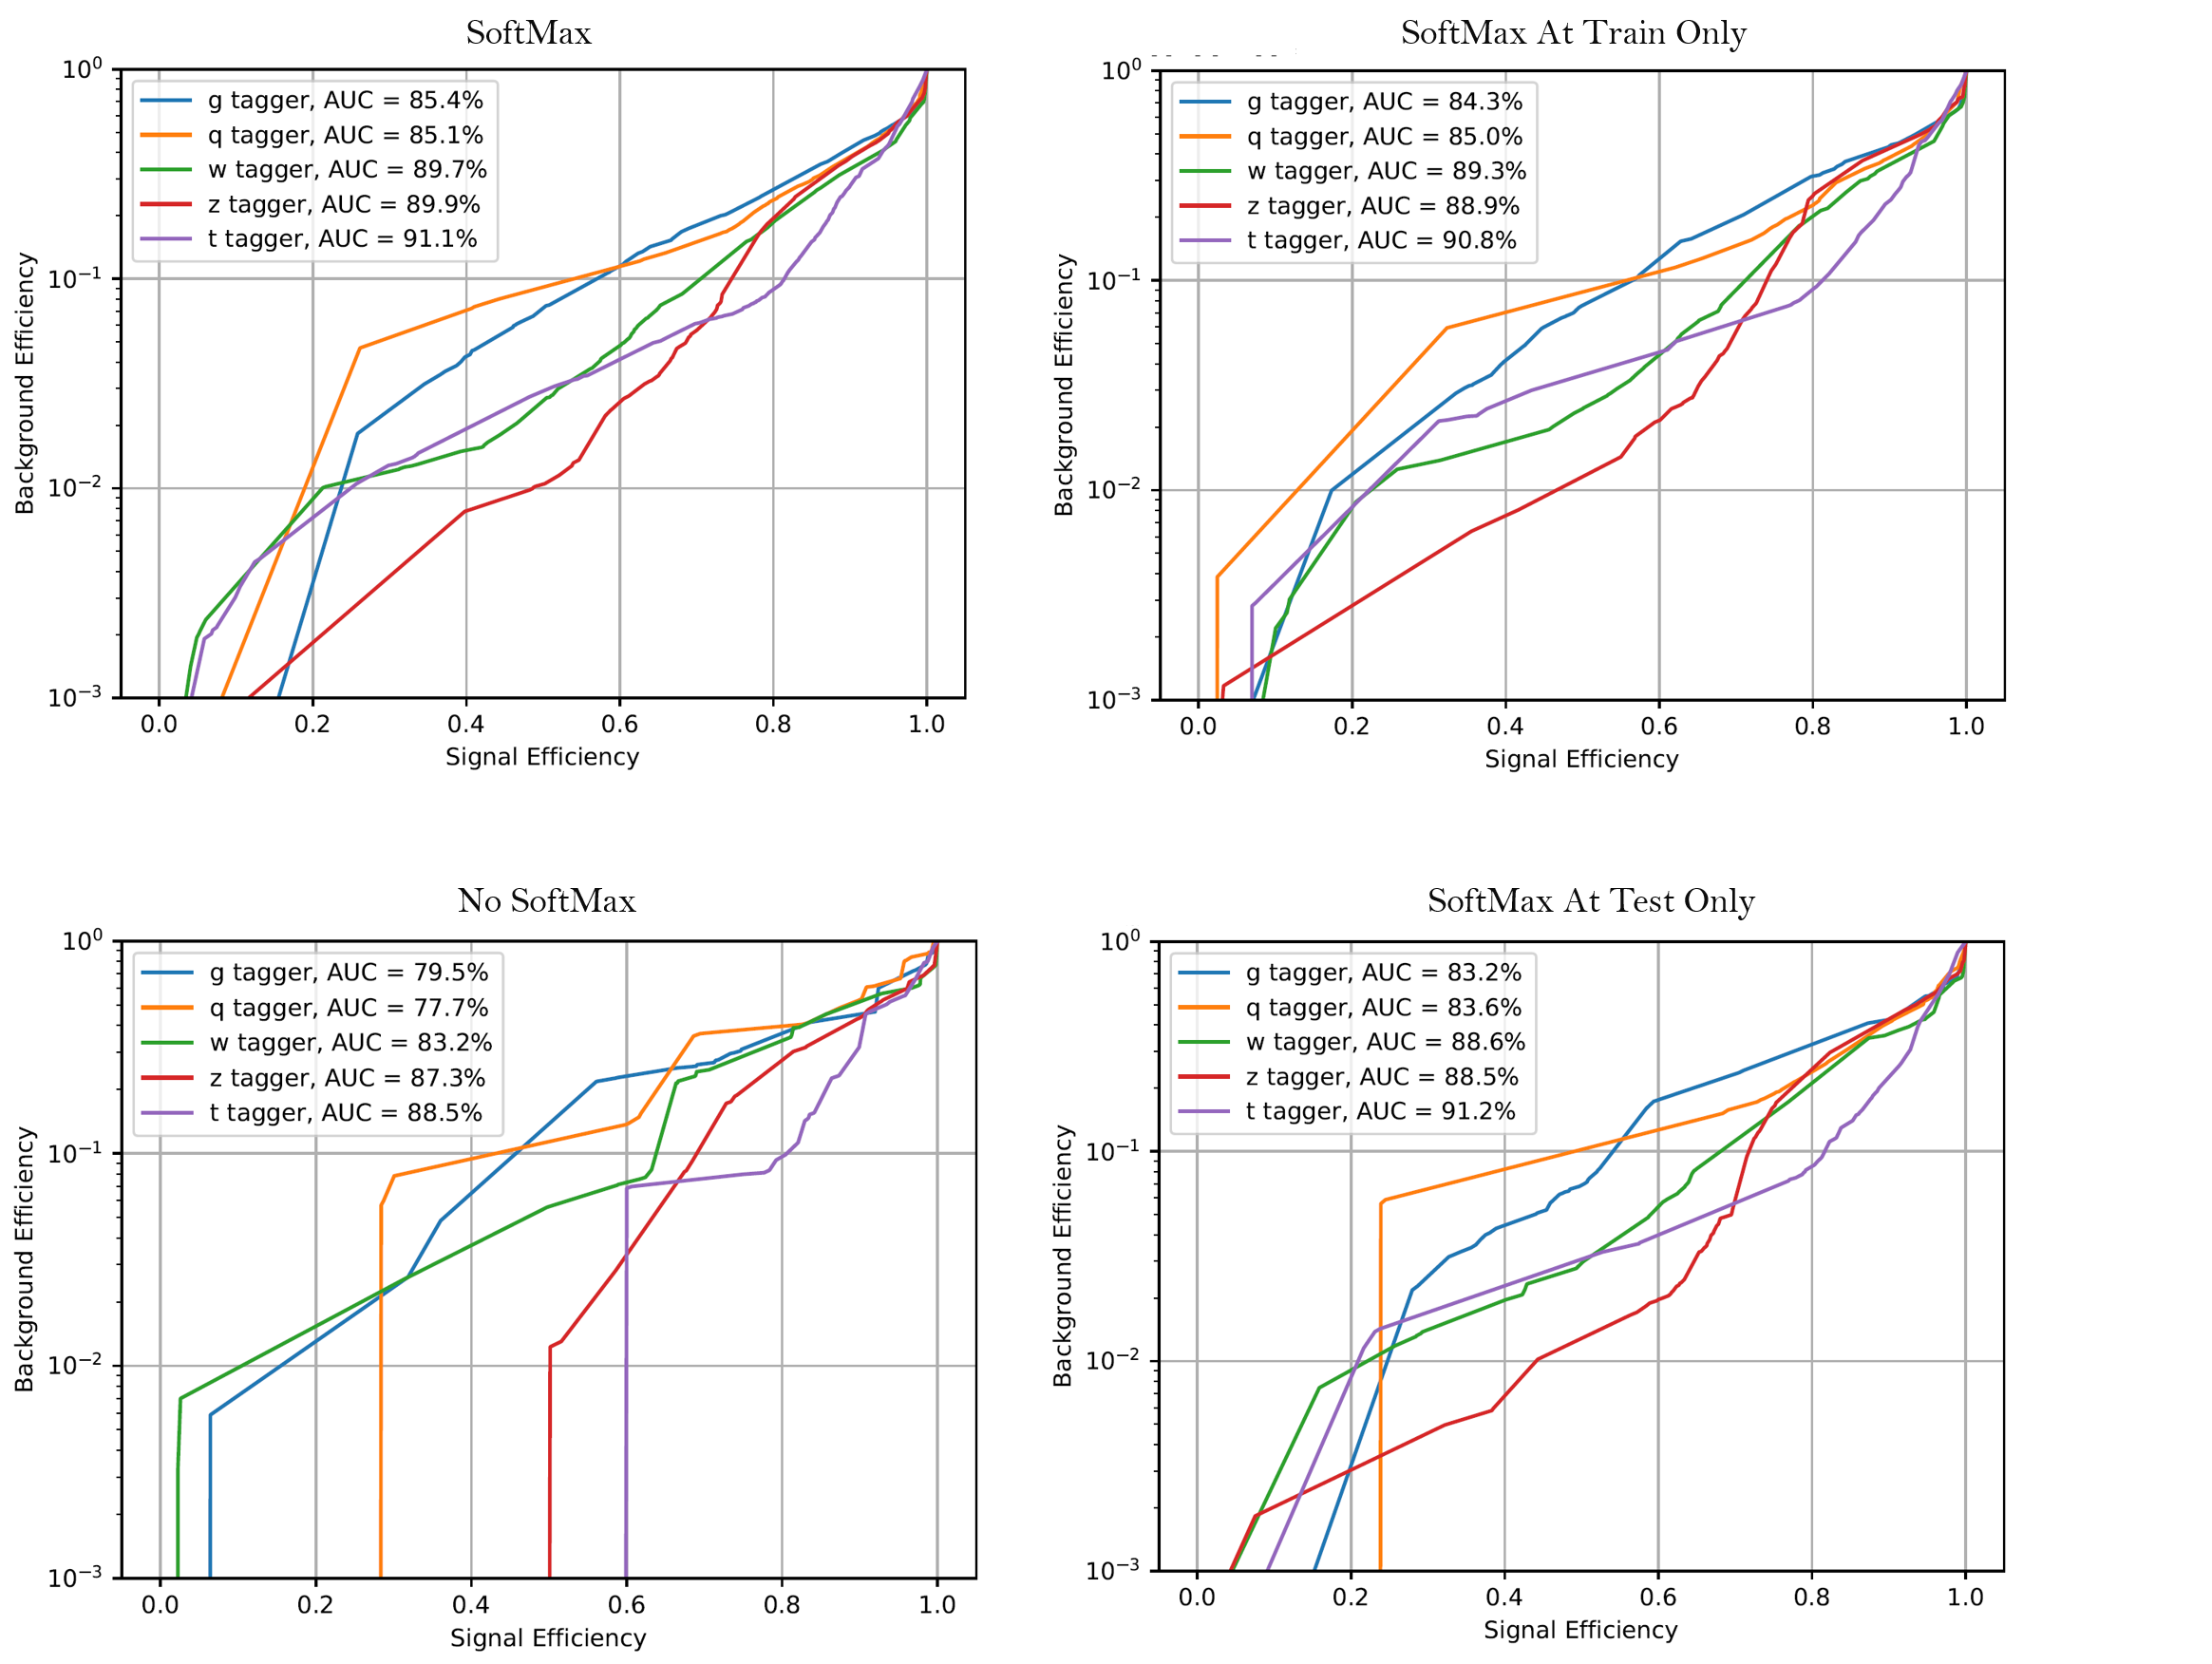
\includegraphics[width=400pt]{figures/bison/SoftMaxTests.png}
%     \caption{We train a model on the FPGA4HEP dataset and observe the classifiers Receiver Operating Characteristics with respect to the SoftMax Layer.}
%     \label{fig:softmaxtests}
% \end{figure}

\newthoughtpar{ROC - Curve and SoftMax}
To test this more closely, we train a model in two ways. The first test is to train a neural network with output quantization, but without SoftMax. We then find its ROC and compare it with the ROC of the same trained model with a SoftMax appended after the final quantizer.The second test is to train a neural network with output quantization followed by a SoftMax. We will then find its ROC and compare it with the ROC of this same trained model but we will drop the final SoftMax layer. This will lend us insights as to whether there is any train time benefits of the final SoftMax layer, additionally also allow us to make claims on whether removing the SoftMax layer from a trained model causes detriments in the ROC of the classifier. 

\newthoughtpar{Exploring the Axes}
To gain further insights into the effects of architectural decisions on the accuracy and LUT costs, we did some elementary grid search.
In Figure \cref{fig:lutvacc}, it is fairly evident that increasing the LUT cost gives higher accuracies. We do however see a clear overlap in two distinct clusters of 'Average AUC-ROC', whereby some models that need very little luts (as less as 2500 LUTs) perform as well as models requiring about 100000 LUTs. Further, we observe that there are some models that require a million LUT, but barely surpass the performance of a model need as little LUTs as 2500. Upon inspection, we discovered that these were models with unreasonably large final layers, or topologies where the per neuron fan-in in bits is too large, while focusing very little on the relationship between Bit-Width and Expand-Size for accuracy.
This becomes more evident in Figure \cref{fig:BWvacc}, where we see that while going from a Bit-Width of 1 to 2 almost undoubtedly reaps benefit. We see diminishing returns when going from bit-width of 2 to 3. While it is not conclusive that increasing bit-width consistently results in diminishing returns, it is still an important insight that we must be aware of the relation between Bit-Width and ExpandSizes. An unwise compromise on one may give sub-optimal results for the same number of LUTs. 

\newthoughtpar{Pruning Techniques}
As discussed in a previous chapter, we have explored many different pruning techniques. While iterative pruning gave the best accuracies, A-Priori Fixed Sparsity was the easiest to train. It thus becomes important to question what utility an Iterative Pruning strategy has over A-Priori Fixed Sparsity, and whether it has any notable benefits for topology exploration. It may be within reason to say that it is worth doing topology exploration using A-Priori Fixed Sparsity, and then taking the discovered topology and training it with Iterative Pruning. It is important to note that at this point of time, the LogicNet Library only supports A-Priori Fixed Sparsity. 
As we can see in \cref{fpganet4hep:tab:iterativeVpriori}, there is a very marginal difference in the \textbf{Average Area Under Curve of the Receiving Operating Characteristic}. 
It thus may be to our benefit to leave topology exploration to A-Priori Fixed Random Sparsity, and use more advanced pruning technique once a suitable topology has been discovered. This claim however is up for further introspection. 


\begin{table}
    \begin{sidecaption}[Iterative vs A-priori Fixed Sparsity]{%
        This table depicts the accuracies for particular models trained with A-Priori Fixed Sparsity and Iterative Pruning techniques. 
    }[fpganet4hep:tab:iterativeVpriori]
\begin{threeparttable}
\begin{tabular}{lrrr}
\hline
Model & LUTs  & A-Priori Fixed Sparsity & Iterative Pruning \\ \hline
A     & 2120  & 88.46                   & \textbf{88.7}     \\
B     & 54060 & 88.96                   & \textbf{89.56}    \\
C     & 59840 & \textbf{88.98}          & 88.92          \\    \hline 
    \end{tabular}
\end{threeparttable}
\end{sidecaption}
\end{table}


% \begin{table}
%     \begin{sidecaption}[Static Mapping Cost]{%
%         Static Mapping Cost to 6:1 LUTs for Fan-In bits.
%     }[st:tab:accuraciesHEP]
%     \centering
%     \begin{threeparttable}
%     \renewcommand{\arraystretch}{1.2}
%     \begin{tabular}{lrrrr}
%         \toprule 
%         HL & BW & X & LUTs & \% Accuracy \\  \midrule\rowcolor{gray!10}

%         6 \            &  1  & 64   &     64   & 100\%    \\ 
%         7\             &  3  & 128  &     192  & 66.67\%  \\
%         8\             &  5  & 256  &     320  & 80\%     \\ 
%         9\             &  11 & 512  &     704  & 72.73\%  \\
%         10 \           &  21 & 1024 &     1344 & 76.19\%  \\ 
%         11\            &  43 & 2048 &     2752 & 74.42\%  \\
%         \bottomrule
%     \end{tabular}
%     \end{threeparttable}
%     \end{sidecaption}
% \end{table}



% /*
% Introduction
% The need for accelerators
%     CPUs, GPUs, ASICs, FPGAs.
% Background
%     FPGA and HW/SW Co-Design
%     Mapping Neurons to Hardware
%       Sparsity
%           Expander, Iterative, Momentum
%       Quantize
%           Activation brevitas
%           Non Linear
% LogicNet: A Library for Mapping HBBs to NEQs
%     Introduction
%     Components
%       Linear
%       Convolutions
%     Design Automation
%       TruthTableGen
%       VerilogGen
%       Synthesis
% Testing LogicNet
%     LogicNet4HEP
%       Introduction
%       Models
%     MNIST 
%       Models
% Concluding Remarks
%     Research Questions
%     Conclusion
% */